% Created 2025-04-08 Tue 22:14
% Intended LaTeX compiler: xelatex
\documentclass[final]{beamer}
         \usepackage[T1]{fontenc}
         \usepackage{lmodern}
         \usepackage[size=custom,width=120,height=91,scale=1.0]{beamerposter}  
         \usepackage{graphicx}
         \usepackage{booktabs}
         \usepackage{tikz}
         \usepackage{pgfplots}
         \pgfplotsset{compat=1.18}
         \usepackage{anyfontsize}



\usepackage{svg}
\usepackage{xcolor}
\usepackage{minted}
\definecolor{bg}{rgb}{0.95,0.95,0.95}
\usetheme{gemini}
\usecolortheme{gemini}
\author{Alán F. Muñoz and Ankur Kumar}
\date{}
\title{Nix for science and fun}
\institute{Imaging Platform, Broad Institute of Harvard and MIT}
\logoright{
\includegraphics[height=3cm]{../logos/broad_logo.png}}
\hypersetup{
 pdfauthor={Alán F. Muñoz and Ankur Kumar},
 pdftitle={},
 pdfkeywords={},
 pdfsubject={},
 pdfcreator={},
 pdflang={English}}
\begin{document}

\begin{frame}[label={sec:org2c7530c},fragile]{}
 \begin{columns}
\begin{column}{0.33\columnwidth}
\begin{block}{Abstract}
One of the biggest challenges for the biological sciences is the replication crisis we face. In addition to inherent biological noise and ever-growing datasets, limited focus on reproducibility of computational processes and their associated results hinders novel discoveries. Improving the reliability and efficiency of scientific research will increase the credibility of current and future scientific literature and accelerate discovery. While there have been improvements in recent years, current technologies fall short of principally solving the problem of software reproducibility. Nix is a framework for software deployment that warrants correct resolution of dependency trees to provide fully reproducible and deterministic packages and environments.
\end{block}
\begin{block}{What is Nix?}
\vspace*{1cm}
\begin{verbatim}
I am unable to re-run your analysis to verify the reported results.

- Reviewer 2
\end{verbatim}

\begin{center}
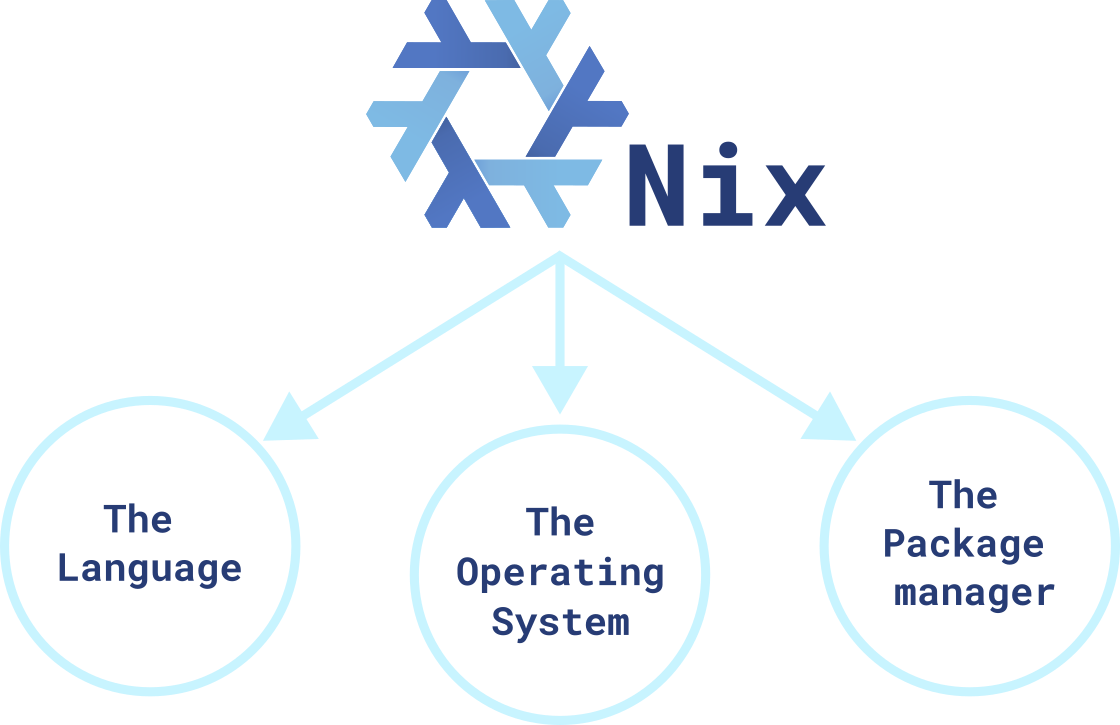
\includegraphics[width=0.6\linewidth]{../figs/nix_trinity.png}
\end{center}
\end{block}
\begin{block}{Problem: Dependency resolution\hfill Solution:}
\vspace*{1cm}
Most package managers and workflow tools are not theoretically sound to provide reproducibility guarantees.
\begin{columns}
\begin{column}{0.5\columnwidth}
\begin{minted}[]{shell}
# Package management with APT on Ubuntu
# Install git system wide
apt install git

# Install CellProfiler via pip
pip install cellprofiler
\end{minted}

\begin{itemize}
\item Packages are installed system wide
\item Version specification is only possible for the top level of the dependency tree
\item Building packages from source is usually not supported or not encouraged
\end{itemize}
\end{column}
\begin{column}{0.5\columnwidth}
\begin{minted}[]{shell}
# Create temporary shell
# with nixpkgs' git
nix shell nixpkgs#git

# Runs cellprofiler 
nix run github:Cellprofiler/
Cellprofiler#cellprofiler
\end{minted}
\begin{itemize}
\item Packages are always isolated and cannot be accessed outside the temporary shell
\item Version specification is possible of the entire dependency tree
\item Packages can be built from source and have first class support
\end{itemize}
\end{column}
\end{columns}
\end{block}
\begin{block}{Problem: Dependency conflicts\hfill Solution:}
\begin{columns}
\begin{column}{0.5\columnwidth}
\begin{minted}[]{shell}
# Install pytorch with cuda 11
apt install cuda-toolkit-11-8

# Install pytorch with cuda 12
apt install cuda-toolkit-12-8
\end{minted}

\begin{itemize}
\item CUDA is installed system wide
\item Cannot install two versions of cuda at the same time without manual symlink and env vars management
\end{itemize}
\end{column}
\begin{column}{0.5\columnwidth}
\begin{minted}[]{shell}
# Create temporary shell with:
# cuda 11
  nix shell nixpkgs#cudaPackages_11.cudatoolkit

# cuda 12
  nix shell nixpkgs#cudaPackages_12.cudatoolkit
\end{minted}

\begin{itemize}
\item Cuda is not installed system-wide
\item Multiple cuda versions can coexist without further environment management
\end{itemize}
\end{column}
\end{columns}
\end{block}
\begin{block}{Problem: Environment replication\hfill Solution:}
\begin{columns}
\begin{column}{0.5\columnwidth}
\begin{minted}[]{shell}
conda env create -f env.yaml
\end{minted}

System wide dependencies cannot be easily shared without containerization.
\begin{itemize}
\item Conda can manage some system libraries, but not all
\end{itemize}
\vspace*{100cm}
\end{column}
\begin{column}{0.5\columnwidth}
\begin{minted}[]{shell}
nixos-shell --flake github:leoank/neusis#oppy
\end{minted}

\vspace*{100cm}
\end{column}
\end{columns}
\end{block}
\end{column}
\begin{column}{0.3\columnwidth}
\begin{block}{Problem: Projects with different requirements\hfill Solution:}
On most operating systems, packages are installed system wide and are not isolated.
This makes it very challenging to work with projects requiring older or newer version of dependencies without breaking the rest of the system.
\begin{columns}
\begin{column}{0.35\columnwidth}
\begin{block}{Normal systems:}
\begin{center}
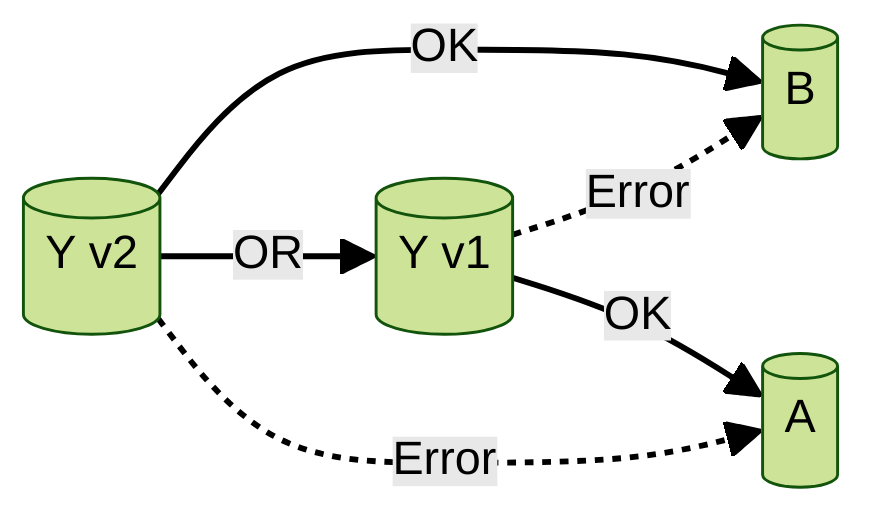
\includegraphics[width=.9\linewidth]{../figs/conflict.png}
\label{}
\end{center}
\end{block}
\end{column}
\begin{column}{0.35\columnwidth}
\begin{block}{Nix:}
\begin{center}
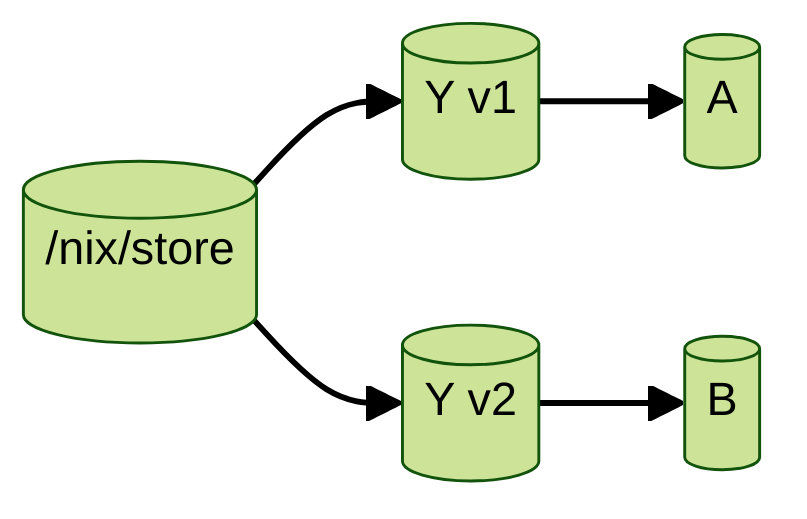
\includegraphics[width=.9\linewidth]{../figs/nix_independent.png}
\label{}
\end{center}
\end{block}
\end{column}
\end{columns}
\end{block}
\begin{block}{Benefits}
\begin{block}{100k+ packages as of April 2025}
\begin{center}
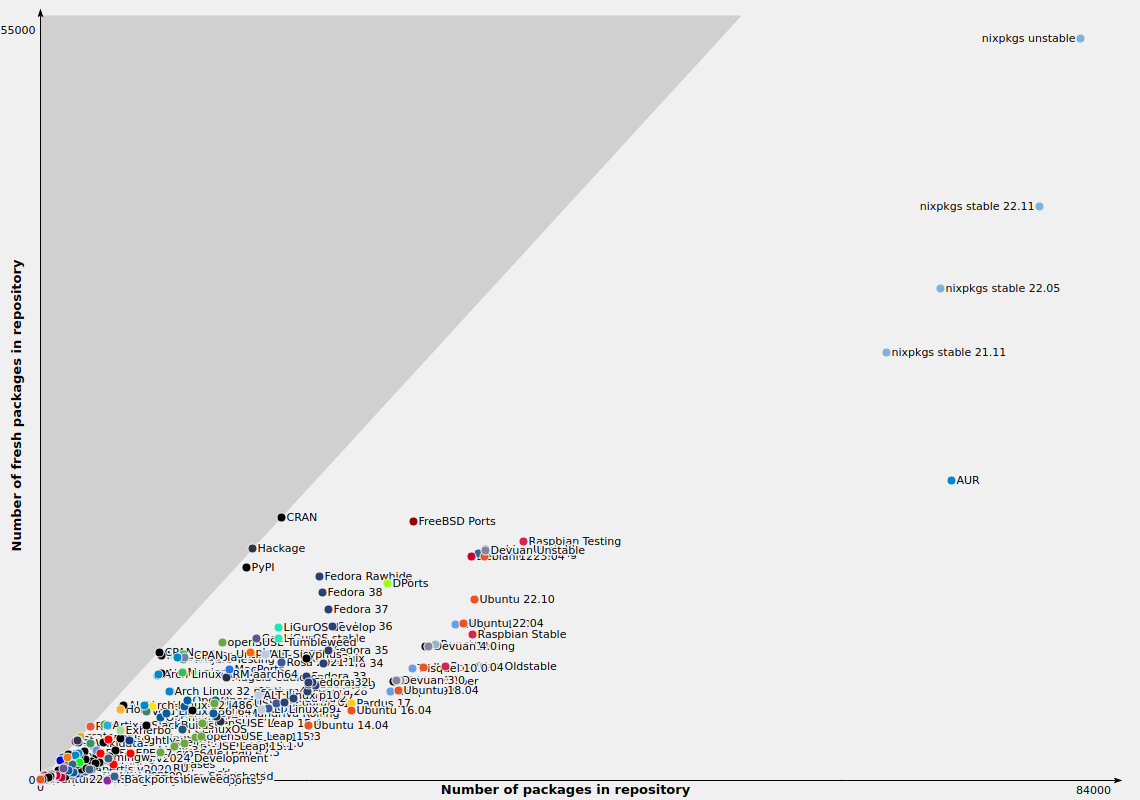
\includegraphics[width=.9\linewidth]{./../figs/npackages_plot.png}
\end{center}
\end{block}
\begin{block}{Consistent environments across different machines and architectures}
\begin{center}
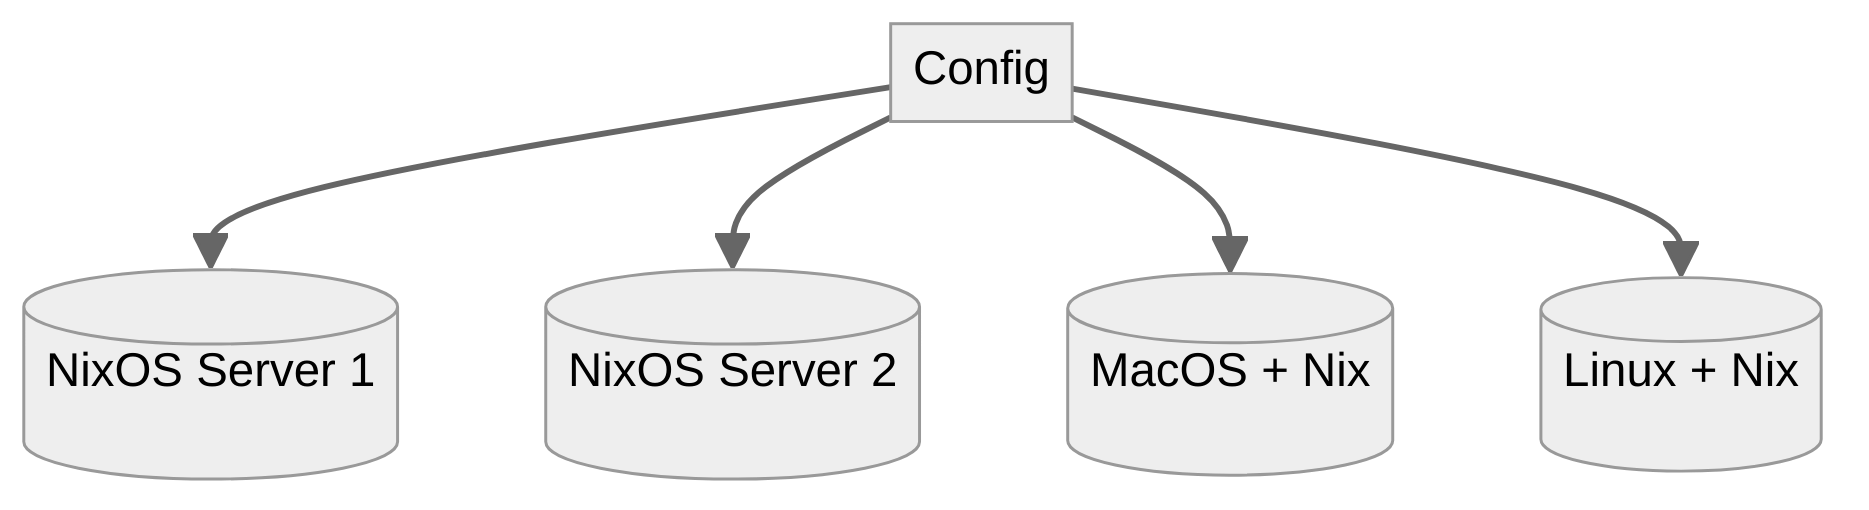
\includegraphics[width=.9\linewidth]{../figs/multiple_machines.png}
\label{}
\end{center}
\end{block}
\begin{block}{Reliably package and deploy software}
\begin{minted}[]{nix}
# file.nix
   {inputs}:
   {
     output = buildPackage{
       unpackPhase = {...};
       buildInputs = {...};
       buildPhase = {...};
       installPhase = {...};
     };
   } 
# $ nix build file.nix
# -> /nix/store/is2vyv9sxn4w9rrgqxg9qhlcf3slfv34-emacs-30.1.drv
# -> /nix/store/is2vyv9sxn4w9rrgqxg9qhlcf3slfv34-emacs-30.1
\end{minted}

\vspace*{100cm}
\end{block}
\end{block}
\end{column}
\begin{column}{0.3\columnwidth}
\begin{block}{Generate entire pipelines with multiple languages and frameworks}
This is useful for updating figures and re-run entire multi-language pipelines becomes a non-issue.

\begin{minted}[]{shell}
#!/usr/bin/env nix-shell
#! nix-shell -i bash --pure
#! nix-shell -I nixpkgs=https://github.com/NixOS/nixpkgs/archive/205a5.tar.gz
#! nix-shell -p bash wget awk R rPackages.Seurat uv

  wget https://remote_data.com/files_of_interest.txt

  awk -f preprocessing_script.awk files_of_interest.txt > preprocessed_data

  Rscript script.R preprocessed_data > new_data
  for pyscript in python_scripts*.py; do
      uv run $pyscript new_data
  done
\end{minted}
\end{block}
\begin{block}{Demos}
\begin{center}

\includegraphics[width=0.7\linewidth]{./../figs/nix_meme.png}
\end{center}
\begin{block}{Run any package in a disposable environment}
\begin{minted}[]{bash}
nix run nixpkgs#inkscape
nix run github:Cellprofiler/Cellprofiler#cellprofiler
export NIXPKGS_ALLOW_UNFREE=1 && nix run nixpkgs#vscode --impure
\end{minted}
\end{block}
\begin{exampleblock}{Ask us for a demonstration!}\label{sec:org474b4a9}
\begin{itemize}
\item Setting up a specific analysis environment
\item Walk me through the CellProfiler derivation
\item Replicate results from a published paper
\item Run a VM configured using NixOS
\item Set up your package of preference
\item Override a package version deep in the dependency tree
\item Set up a flake for a reproducible environment
\item Help me set up Nix package manager on my system
\end{itemize}


Also reproduce your entire home environment in other computers, across Linux, Windows, MacOS and Android*
\end{exampleblock}
\end{block}
\begin{block}{Additional resources and links}
\begin{center}

\includegraphics[width=0.4\linewidth]{./../figs/qrcode.png}
\end{center}

\vspace*{100cm}
\end{block}
\end{column}
\end{columns}
\end{frame}
\end{document}
